\white{Programming (May 15, 2024)}
\label{Programming}
\chapterauthor{Ian Smith}
\info{Caleb Bachmeier}{Programming}{May 15, 2024}
\textbf{Goal}: Explain Ian's programming work

\section*{Introduction}
The challenges of this year's game require a unique and nuanced approach to programming. While traditional programming remains largely similar to previous years, skills programming is significantly different due to the placement of game objects and the scoring requirements.

\section*{Skills Rules}
Skills Rules are explained in detail in the previous chapter: \blueref{skills-rules}{Skills Rules}
\section*{Programming Skills Challenges}
Some of the most unique challenges, after analyzing programming skills challenges, are the requirements to create a program that can list all the ways to earn skills points.

\section*{Proposed Solutions}
Some of the proposed solutions included using standard programming techniques with basic VEX functions similar to previous years, employing a repeating program developed by Ian in earlier seasons, implementing LemLib for PID and Pure Pursuit control, utilizing AI for autonomous control, and combining LemLib with AI. Due to the potentially significant rewards of the last option, that approach was ultimately developed.

\section*{AI Development}
Ian's AI development is explained in full detail in chapter \blueref{Artificial-Intelligence-Library}{Artificial Intelligence Library}

\section*{General Match Control}
In terms of general match control, several key points have emerged so far this season: a HUD for the robot brain and options for improved control.

\section*{Control System}
After testing curvature drive and arcade drive with our driver(s), we determined that curvature drive offers better control. The concept of curvature drive allows the robot to follow a fixed radius curve based solely on the steering stick, eliminating reliance on velocity like arcade drive.

\section*{HUD Design}
For HUD design, several concepts were considered, including an interactive terminal and interactive menus. Due to the simplicity of the menus and their ease of programming, that option was chosen.

\section*{Programming Software}
All programming is conducted on Ubuntu, as it was the system I had available. The PROS software was the obvious choice over the VEX V5 name-space and compiler due to its closer adherence to C standards and versatile features.
\begin{comment}
\white{Fusion 360 (May 16, 2024)}
\label{Robot-CAD}
\chapterauthor{Connor Albers }
\info{Caleb Bachmeier}{Fusion}{May 16, 2024}
\textbf{Goal}:
    \section*{Robot CAD}
\end{comment}
\important{CNC Machining Research (May 17, 2024)}
\label{CNC-Machining}
\chapterauthor{Ian Smith}
\info{Ian Smith}{CNC Machining}{May 17, 2024}


\textbf{Goal}: Explain the team's CNC machining research

% CNC Machining Research
\section*{CNC Machining (Research)}

% Introduction and Background
\subsection*{Introduction and Background}
After brief experimentation last year with using primitive (mostly “eyeballing”) methods of custom parts manufacturing and “machining” —used very loosely,— we have decided to take advantage of the resources available to us. Fortunately, our team coach, Paul, is a hobbyist machinist with a relatively diverse range of tooling. Among the tools are mills, lathes, and a 4-axis CNC mill. However, to maintain VEX legality, a few rules must be followed.

% VEX Legality
\subsection*{VEX Legality}
Because of rule \textless R2\textgreater, it has to be members of our team doing the machining. This includes all CAD, tool-path generation, G and M code generation, calculations, and machining operations.

Machining (including CNC) is legal because it is subtractive manufacturing and is only modifying the VEX part, which is legal per rule \textless R16\textgreater: "Physical modifications, such as bending or cutting, of legal metal structure or plastic components are permitted.".

% Resources and Stock
\subsection*{Resources and Stock}
Primarily, as resources for the project, we used suggestions from our coach along with the \textit{Machinist’s Handbook}. Regarding our “stock,” we are relatively limited, with only high-strength axles (SKU 276-7465) and 24-tooth gears (SKU 276-7572) making convenient stock. High-strength axles are synonymous with Zinc Galvanized ¼ inch Square Stock with a maximum length of 24 inches. The 24-tooth gears are synonymous with 0.9-inch diameter round stock with a maximum length of ½ inch. Both parts are assumed to be 1045 mild steel based on what we found on the VEX website. Overall, the material is quite limiting, but we are still capable of making custom small-space mechanisms. One of the theorized applications of machined parts was custom gearing through better build mechanisms such as steel helical gears with custom ratios. 

% Research and Calculations
\subsection*{Research and Calculations}
When researching the stock to find relevant information, I started by going to McMaster-Carr to find the corresponding square stock (\href{https://www.mcmaster.com/8962K33/}{This is a link to McMASTER-CARR}). Afterward, I found a stress-strain graph for the alloy to perform calculations on the material when engineering custom parts (\href{https://www.mdpi.com/2073-4352/13/8/1287}{This is a link to the project page}
\textcite{cryst13081287}).

\begin{figure}[H]
    \centering
    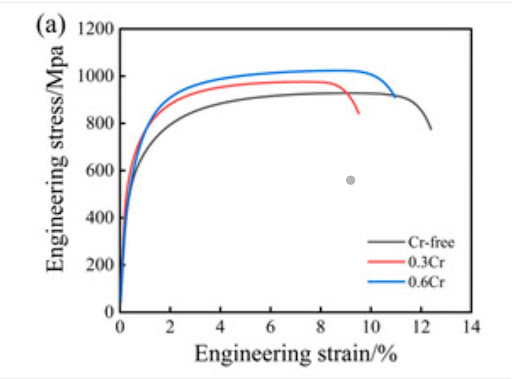
\includegraphics[width=0.5\linewidth]{images/CNC Machining Graph.jpg}
    \caption{Engineering Strain \%}
    \label{fig:cnc-machining-graph}
    \cite{cryst13081287}
\end{figure}

After interpreting the graph, we observed a yield point at about 800 MPa/mm\(^2\). After discussion, we decided to maintain a factor of safety around 1.5, or aircraft grade. This was decided because we don’t need longevity; we need short bursts of performance from our parts. The only downside to that low of a factor of safety is the occasional extreme forces our robots may be subjected to during a match. The most likely stress we will have to engineer around is shear force. For our stress calculations on parts, we plan on using the tool within Fusion 360, which we use to design the bot for construction, testing, and simulation.

\section*{Clarification on Legality}\footnote{Added: November 18, 2024}

At our North Dakota Signature Event, despite the repetitive clarifications on legality, we were still questioned about rule violations. As a solution to this problem, we were posed with a few different solutions. We could go back and edit the original entry. We could clarify in a different entry. We could add an FAQ to the original entry. We decided to go with the last option because of the clarity and simplicity. 

\begin{itemize}
    \item \textbf{Are you using non-VEX legal parts?} \\
    No, we are not using non-VEX parts. We actually haven’t bought a part to machine yet.
    
    \item \textbf{Have you machined a part yet?} \\
    No, we have not machined a part yet, we technically haven’t bought stock yet.
    
    \item \textbf{Based on this research, how did you derive material type?} \\
    Experience outside of VEX. The 1045 Low Carbon Steel comes directly from the VEX Website "\cite{vexRobotics}", which is backed up by \textit{\textit{Machinery’s Handbook} "\cite{machinists}."} "\cite{machinists}." The Zinc/Chromium plating comes from assumed corrosion resistance and the shiny material on the outside of the shaft.
    
    \item \textbf{Why are you citing an outside purchasing source (McMaster-Carr)?} \\
    Before I knew \textit{Machinery’s Handbook} "\cite{machinists}." existed, I took the information I knew about material science and also knew that I didn’t have enough information to do full stress calculations. I just went onto a third-party source and looked for ¼ inch 1045 square stock. Because of VEX’s lack of information and my not owning a copy of \textit{Machinery’s Handbook} "\cite{machinists}." yet, I had to go to an outside source for research purposes only.
    
    \item \textbf{How will you document the work process?} \\
    We plan on recording the process of writing the G and M codes, documenting the math used before the operations, and recording the actual machining. On the condition that we are asked by a Judge or Referee at an event, our goal is to be able to show undisputable evidence that everything we did was completely legal.
\end{itemize}

In conclusion, this short FAQ was intended to show that the chapter was written as research only and we always have purchased legal parts.
